\part{Computing System}

计算机(Computer)是一种设备,并且计算机有通用机和专用机之分,而计算系统(Computing System)则是一种动态实体,用于解决问题以及与它所处的环境进行交互。

计算系统由构成设备的硬件、机器执行的软件程序及由前两者管理和操作的数据构成,计算系统可以分为多个层次。

\begin{compactitem}
\item 计算机硬件(Computer Hardware):指计算系统的物理元件集合。
\item 计算机软件(Computer Software):指提供计算机执行的指令的程序集合。
\end{compactitem}

计算系统就像一个交响乐团,把许多不同的元素组织在一起,构成了一个整体,但这个整体的功能却远远大于各个部件的功能总和。

计算系统的核心是它管理的信息,如果没有数据,硬件和软件都毫无用处。

在计算机科学中,计算机其实就是:接收用户输入指令与数据,经过中央处理器的数据与逻辑单元运算处理后,以产生或存储成有用的数据。

\chapter{计算系统的分层}

有关计算机体系结构的不同定义可以建立在四个基本概念之上,它们是结构、组成、实现和性能。其中,
\begin{compactitem}
\item 结构定义了各个硬件部件之间的互连;
\item 组成定义了各个部分之间的动态相互影响和管理;
\item 实现定义了硬件部分的详细设计;
\item 性能说明了计算系统的行为。
\end{compactitem}

计算系统也可以通过处于若干抽象层之间的接口加以定义,其中每一层将为它的上一层提供功能支持,这些层包括应用程序、高级语言和机器指令集。

根据系统不同级间的接口,就可以定义不同的计算机体系结构。处于应用程序和高级语言之间的接口称为语言体系结构。指令集体系结构定义了基本指令集和运行时间及I/O控制之间的接口。

计算系统可以比作洋葱,它们的相似之处就是它们的内部结构都是一层层的。通过采用自底向上,由内至外的方式,可以通过抽象将计算系统分为6层,分别是信息层、硬件层、程序设计层、操作系统层、应用程序层和通信层,注意这里的每一层都是抽象层,这种划分顺序又称为自底向上。这样就像剥离洋葱分层一样剥离计算系统的每一层,可以理解为计算系统由这些抽象层构成,而每个抽象层在整个系统设计中都扮演了一个特定的角色。
\begin{figure}[!h]
\centering
\caption{计算系统分层}
\label{计算系统分层}
\begin{tikzpicture}

\filldraw[draw=gray,fill=magenta] (5,2.9) ellipse (2 and 2.8);
\filldraw[draw=gray,fill=cyan] (5,2.5) ellipse (1.4 and 2.3);
\filldraw[draw=gray,fill=blue] (5,2.2) ellipse (1.1 and 2);
\filldraw[draw=gray,fill=green] (5,2.05) ellipse (0.8 and 1.7);
\filldraw[draw=gray,fill=red] (5,1.7) ellipse (0.5 and 1.3);
\filldraw[draw=gray,fill=lightgray] (5,1.45) ellipse (0.3 and 1);
\draw[loosely dashed] (5,0)--(5,6);

\draw (5.1,0.7)--(7,1.2)--(8,1.2) node[right] {信息层}; 
\draw (5.35,1.2)--(7,1.8)--(8,1.8) node[right] {硬件层};
\draw (5.65,1.75)--(7,2.4)--(8,2.4) node[right] {程序设计层};
\draw (5.95,2.4)--(7,3)--(8,3) node[right] {操作系统层};
\draw (6.2,3)--(7,3.6)--(8,3.6) node[right] {应用程序层};
\draw (6.4,3.8)--(7,4.2)--(8,4.2) node[right] {通信层};

%\caption{计算系统分层}
\end{tikzpicture}
\end{figure}

计算机和它的机器语言构成了洋葱的芯,软件层和更复杂的硬件一层层地裹住了这个芯。由机器语言、汇编语言、FORTRAN、Lisp、Pascal、C、C++和Java等程序设计语言以及使用这些语言进行的程序设计构成了程序设计层。操作系统和它的资源管理技术(包括更大、更快的二级存储介质上的文件)包围着这些程序,并对它们进行管理。

接下来的一层由更复杂的通用或专用软件系统构成,它们覆盖了操作系统,而且操作系统与硬件有相当程度的关联性。这些功能强大的程序由并行理论支持。最后一层由网络和网络软件构成,网络软件包括计算机之间通信必需的所有工具,他们最终组成了现在的Internet和万维网。

当这些层随着时间的流逝逐渐增长时,用户对计算机系统的硬件接触的越来越少。每个层都是它下面的计算机系统的抽象。

当我们把计算分层逐个地从计算系统中剥离出来,每次只探讨一个分层,每个分层自身就不那么复杂了。事实上,计算机真正所做的只是非常简单的任务,它盲目地快速执行这些任务,根本不知道可以把许多简单的任务组织成较大的复杂任务。

了解了计算机系统,就可以探讨计算机如何运作,它可以做什么以及如何做。当人们把这些计算机的抽象分层组织在一起,让它们各自扮演自己的角色,这种简单组合产生的效果是惊人的。

计算的历史被划分为四个时代,每个时代都以用于构建硬件的元件和为了让用户更好地利用这些硬件而开发的软件工具为特征,这些工具构成了包围硬件的软件层。

最内层也是最底层的信息层反映了在计算机上表示信息的方式,它是一个纯概念层。计算机处理的信息采用二进制数字0和1管理。要了解计算机处理技术,必须了解二进制数制以及它和其他数制之间的关系,然后就可以通过获取其他类型(如数字、文本、图像、音频和视频等)的信息,进一步理解各种类型数据以及如何用二进制格式表示它们。

接下来的硬件层由计算机系统的物理硬件组成,计算机硬件包括的设备有门和电路,它们都按照基本原理控制电信号,正是这些作为核心电路,使专用的元件(如CPU和存储器)得以运转。可以这样理解,硬件层的工作就是处理由0和1组成的数字信号。

程序设计层负责处理软件、用于实现计算的指令及管理数据,程序有多种形式,可以在许多层面上执行,由各种语言实现。尽管程序设计问题多种多样,但是它们的目的是相同的,即——解决问题。程序设计就是设计算法以高效地处理数据,解决问题。

现代计算机都用操作系统(OS)管理计算机的资源,比如UNIX、Windows、Linux和Mac OS等。操作系统管理计算机的所有资源,使用户与计算机系统进行交互,管理硬件设备、程序和数据间的交互方式。了解操作系统为我们做了什么,通常是理解计算机的关键。

上述分层的重点在于使计算机系统运转,而应用层的重点则是用计算机解决真实世界的问题,通过运行应用程序在其他领域利用计算机的能力,如进行建筑设计、开发游戏等。

不同领域涉及的专用计算机软件工具范围广大,涉及计算学的几个子学科,包括信息系统、人工智能、仿真等。

通信层作为计算系统操作的基础层,使得计算机可以相互之间进行通信,从而不再是某个人桌面上的孤立系统。通过通信层使得计算机可以接入到网络中来共享信息和资源,Internet逐渐演化成了全球性的网络,利用计算技术可以与地球上的任何地方通信,这从根本上改变了计算机的使用价值,使计算机普及到一般大众。

World Wide Web使通信变得相对容易,计算机通信层的协议是一套规定必须严格遵守的规则和(交互信息的)过程的代码,在计算术语中借用它来表示计算机在进行交互的时候使用的正确规定。

最后,除了讨论计算机能够做什么以及如何做的,我们还要讨论计算机不能做什么,或者至少不能做的很好。

计算机在表示信息方面有其固有的缺陷,程序设计只能尽可能地改善这一点。另外,还有一些问题是根本不能解决的,通过这些,也说明了计算机系统的缺陷。

\chapter{抽象}

将计算系统进行分层,实际上是对计算系统的一种抽象(abstraction)。

抽象是一种删除或隐藏了复杂的细节的心理模型,是一种思考事情的方式。抽象后就只保留了实现目标所必需的信息。例如,在与计算机的一个抽象分层打交道时,没有必要考虑其他的抽象分层。同样道理,在编写程序时,不必关心硬件是如何执行指令的,而在运行程序时,也不必关心程序是如何编写的。

大量的实验表明,人在短期记忆中可以同时管理大约7条(根据个人情况,可以增加或减少2条)信息,这称为Miller定律。

Miller定律显示,当我们需要其他信息时,可以得到它,但当我们集中于一条新信息时,其他的信息就会退回二级状态,同样当我们与计算机的一个分层打交道时,没有必要考虑其他分层。

这个概念就和变戏法的人能够同时在空中保持的球数是相似的,人的智力只能玩7个球,当我们拾起一个新球时,必须抛掉前一个球。虽然7看起来是个很小的数字,但关键在于每个球可以表示一种抽象,或者一大块信息,也就是说,我们抛的每个球都可以表示一个复杂的论题,只要我们把它看作一种想法即可。

在日常生活中充满了抽象,例如,要开车出去,我们不需要知道车是如何运转的,也就是说,我们根本不必详细地知道引擎是如何工作的,而只需知道一些驾驶的基础知识,即如何与车互动以及如何操作踏板、手柄和方向盘即可,甚至不必同时考虑这几个方面。而且即使我们知道引擎是如何工作的,在开车的时候也不必考虑它,一部汽车太复杂,我们不能同时关注它的所有方面,这些技术细节就像变戏法时抛起的球,同时想关注所有技术细节就太多了,但是,如果能够把汽车抽象成较小的规模,使我们能与之交互,那么就可以将它作为一个实体处理,此时,无关的细节将被忽略。

如其名所示,抽象艺术是另一种抽象的例子,一幅抽象画确实表示某些东西,但绝不会陷于事实细节的泥沼。

抽象是计算的关键,计算系统的分层表现了抽象的概念,而且,抽象还以各种形式出现在各个分层中,而且在计算系统的整个演化过程中都有抽象的影子。

1936年,由英国数学家Alan M.Turing发明的图灵机就是一种抽象数学模型,本质上它与硬件毫无关系,图灵机为计算理论的主要领域奠定了基础,分析图灵机的功能是所有学习计算机科学的学生的理论学习的一部分。

\chapter{计算工具}

计算机的出现和发展,在一定程度上满足了当时的生产和科学技术各部门所提出的计算任务要求,但这些计算工具只能简化人的手工计算,也就是说计算机只是解决了人们对于“需要计算什么”的看法,而计算的方法和计算步骤地提出、计算过程的控制、数据整理等主要还是靠人制定相应的规则来指示计算机执行。

计算机可以认为是,接收用户输入的指令和数据,经过中央处理器的数据和逻辑单元处理后,以产生或存储成有用的信息。


隐藏在所有计算问题之下的基本问题是“什么可以被有效的自动操作?”

到底谁在把计算机用作工具?现在除了为其他人创建工具的程序员之外,所有人都在使用计算机这个工具。对于那些工具制作者来说,计算是一种学科(低级工具),或者计算这种学科使它们的工具成为可行的(将一种应用程序构建在另一种应用程序之上)。

系统研究带来了更好的通用工具,应用研究为领域特定的应用提供了更好的工具,而且毫无疑问,把计算主题直接作为学科研究的人将影响那些把计算机用作工具的人,计算研究促成了人们日常使用的应用,而技术转变的速度也惊人的快,这种共生关系在计算学中比在其他学科中更强。

\chapter{计算学科}

学科(discipline)被定义为一种学习领域,Peter Denning把计算机科学学科定义为“计算机专家在工作中使用的知识和实践的主体,这一学科也称为计算机科学和工程学,计算学或信息学”,“计算知识的主体经常被描述为对算法过程的系统研究,包括算法的理论、分析、设计、有效性、实现和应用”。

关于计算学是一种数学学科,还是一种科学学科或工程学科,存在着长期的争论。

计算学来源于数理逻辑,通过图灵定理可知,有些问题是不能解决的。Boolean理论描述了计算机电路,数字分析在科学计算机中扮演着重要的角色。
科学学科在尝试理解它们的系统是如何运作的,而自然科学的存在是为了“填写上帝忘记给我们的说明书”,因此,在构建和测试自然现象的模型时,计算学属于科学学科,在设计和构建计算系统时,采用的则是工程学的技术。
Peter Denning认为每个计算机科学从业人员都需要四个领域的技巧。

\begin{compactitem}
\item 算法思想,即能够用按部就班的过程表示问题,从而解决它们;
\item 表示法,即用能被有效处理的方式存储数据;
\item 程序设计,即把算法思想和表示法组织在计算机软件中;
\item 设计,使软件满足一种用途。
\end{compactitem}

1989年提出的一种计算机科学课程模式认为,计算机科学学分为以下的三个方面:理论(数学)、抽象的实验(科学)和设计(工程学),其中:

\begin{compactitem}
\item 理论(数学)指为理解一个领域中的对象之间的关系而构建的基本概念和符号;
\item 实验(抽象)指研究不同应用领域内的系统和体系结构的模型,判断这些模型是否预测了新的行为;
\item 设计指构造支持不同应用领域内的工作的计算机系统。
\end{compactitem}

按照这三个方面可以分为12个分区,其中有6个与理解和构建计算工具有关,它们是算法和数据结构、程序设计语言、(计算机)体系结构、操作系统、软件方法学和工程学以及人机交互,它们同时也被称为系统分区,另外的6个分区则与计算机作为工具的用途相关,分别是数值和符号计算、数据库和信息检索、人工智能和机器人技术、图形学、组织信息学及生物信息学,这些分区被称为应用分区。

\begin{table}[htbp]
\centering
\caption{计算机科学的分区}
\label{计算机科学的分区}
\begin{tabular}{|p{110pt}|p{110pt}|p{110pt}|}
\hline
算法和数据结构 & 操作系统 & 人机交互	\\
\hline
程序设计语言 & 软件方法学和工程学 & 图形学	\\
\hline
体系结构 & 数据库和信息检索 & 组织信息学	\\
\hline
数值和符号运算 & 人工智能和机器人技术 & 生物信息学 \\
\hline
\end{tabular}
\end{table}

\section{计算机科学}

计算机科学与其说是关于计算机的科学,还不如说是用计算机解决问题的科学。计算机本身只是计算机科学的一部分,而问题求解才是计算机科学的一个重要组成部分。

计算机只是有形的实体,作为一种通用的机器,现代计算机具备执行许多任务的潜力,但必须对其编程(programmed)才能挖掘出这种潜力。给计算机编程就是给它一组指令,即一个程序,这组指令详细指明解决问题的每一个必要步骤。这些程序通常被称为软件(software)。

只有软件和硬件结合在一起,计算机才能进行指定的计算。与计算硬件相比,软件是一个抽象的、无形的实体。软件是用硬件能够解释的准确语言所表述的一系列简单步骤和操作过程。

计算机软件和用计算机解决问题的活动,是计算机科学的核心。当谈及计算机科学时,我们主要关心的是计算机软件领域,更重要的是抽象的问题解决领域。从许多方面来看,最好将计算机科学看作解决问题的科学,而现代解决问题的工具离不开计算机。

\section{计算机科学与交叉学科}

由于计算机/信息技术和生物技术出现了交点,所以出现了综合两者的技术。其中一个领域就是生物信息学,它涉及用计算机和计算机网络获取、存储、处理、分析、虚拟化和共享生物信息。

许多生物研究(包括遗传和染色体在内)现在都是通过计算技术和建模技术(也就是使用生物物质的数字表示法)来执行的,而不是采取化学方式执行的传统的“湿”实验室技术。到2003年为止,染色体研究已经可以用计算机工具绘制完整的人体染色体组。如果使用传统的排序方法,还需要更多年来实现这一目标。计算技术还帮助研究员定位了许多疾病基因,这一成果使治疗和治愈这些疾病的制药业飞速发展。不过,在遗传和染色体研究中采用计算机技术还存在一定的争议,例如deCODE Genetics公司这个案例。

\section{算法}

由于计算机科学是在计算机的帮助下解决问题的学科,所以应该了解算法(algorithm)的概念。这个概念无论对计算机科学还是对解决问题的抽象学科来说都是基础。通俗地说,算法是一种解决问题的策略,下面将这种直观的理解正式化并给出严格定义。

要成为一个算法,解决问题的技术必须满足三个基本要求。

首先,算发必须用清楚地、明确的形式来表达,以使人们理解其中的每一个步骤。

第二,算法中的每一个步骤必须有效,以便人们在实践中能够执行它们。例如,若某一个算法包含“用$\pi$的确切值与r相乘”这样的操作,则这个算法就不是有效的,因为无法算出$\pi$的确切值。

第三,算法不能无休止地运行下去,而必须在有限的时间内给出一个答案。

简而言之,算法必须是:

\begin{compactenum}
\item 清楚、明确地定义。
\item 有效,即每一步骤都切实可行。
\item 有限,既可以在有限步骤后得到结果。
\end{compactenum}

总之,算法是种抽象的解决问题的策略,这种策略最终将成为所编写的程序的核心。与所要解决的问题一样,算法在复杂性上差别很大。在大多数情况下,解决一个问题可以使用几个不同的算法,在编写最终程序之前需要考虑许多潜在的解决方案。


\chapter{计算简史}

在计算机工业的发展过程中,从一开始就要指出建造计算机并不是源自一处,有充分的理由相信,建造第一台计算机的尝试存在于地球的不同地方,而且建造计算机更需要合作。

从某种意义上说,计算的使用古已有之,许多早期数学家致力于解决重要的实际问题的计算,比如观察兽群中动物的数量,计算小块土地的面积或记录商业交易等。这些活动要求人们开发新的计算技术。例如,算盘这种计数装置大约于公元前2000年就出现了。

纵观计算的历史,计算的发展相对来说较为缓慢。1623年,德国科学家Wilhelm Schickard发明了第一台机械计算器,可以自动执行简单的算术计算。由于三十年战争(1618$\sim$1648)的破坏,Schickard的发明已经失传。

法国哲学家Blaise Pascal于17世纪40年代用类似的技术发明了机械加法器,其复制品现存于巴黎。

1673年,德国数学家Gottfried Leibniz发明了一种相当复杂的装置,除进行加减运算外还可以进行乘除运算。所有这些装置都是纯机械的,没有发动机和其他动力源。操作者通过将金属轮转到特定的位置来输入数字,而转动这些金属轮又可带动机器的其他部分,从而改变显示的结果。

工业革命期间,人们开始考虑使用蒸汽机驱动更复杂的计算机器,这种机器可在自己的动力控制下进行复杂的计算。在这一领域中,有突出贡献的是英国数学家Charles Babbage。

Babbage一生中设计了两种不同的计算器,分别称为差分机和分析机,分别代表了当时计算器所取得的巨大进展。可惜的是,他没能完成这些项目。其中用于产生数学函数表的差分机直到1854年才由瑞典发明家实现。

在Babbage的设计中已经包含了现代计算机的许多基本特点。最重要的是,在Babbage的构思中,分析机是一种通用的机器,可根据设计好的程序实现许多不同的功能。在这个设计中,分析机的操作是由一张卡上的一组小孔来控制的,机器可以读出这组小孔的排列模式。通过改变小孔的排列模式,人们可以改变机器的行为,从而执行不同的运算。

人们对Babbage的工作的了解主要来自Augusta Ada Byron,Ada预见到分析机的潜力,并为这种机器设计了一些复杂的程序,因而成为第一个程序员(Programmer)。

Babbage的一些设计理念在很大程度上影响了其后的计算发展,例如,用穿孔卡片控制计算,这种想法最初是由法国发明家Joseph Marie Jacquard提出并运用于自动织布机上的。1890年,Herman Hollerith用穿孔卡片为美国人口普查数据自动生成报表。

直到20世纪40年代,电子学的出现才使超越一直占统治地位的机械计算器的梦想实现,实现了Babbage关于可编程的计算机的梦想。

较为公平的说,第一台程序控制(机械)计算机是Z1(1938年),接着在1939年出现了第一台定点算术操作程序控制计算机Z2。

按我们现今对黑客的定义,德国工程师克兰德·楚泽(Konrad Zuse)其实并不能算上是一位黑客。但若没有他的存在,黑客这个词的出现就会被向后推迟若干年,人们称他为数字计算机之父,因为是他发明了世界上第一台具有完备程序控制功能的数字计算机——Z3。楚泽最初在父母的房屋内开始组建Z3的初代——Z1,并于1938年完成。楚泽获得了当时德国政府的资金支持,于是他将Z1计算机一步步完善,最终在1941年完成了数字计算机鼻祖——Z3的制造。受限于当时混乱的二战,楚泽无力将数字计算机升级为电子计算机。

在大学中,第一次有记载的建造计算机的尝试可以追溯到20世纪40年代早期(1939年)的美国依阿华州立大学,该大学的研究者John Atanasoff想出了如何构造高效电子计算机,他认为这是一种电子设备,能够直接进行逻辑计算,而不是像模拟设备那样,需要列举。它使用的是二进制数,而不是十进制数,内存使用电容器,用再生处理避免漏电造成的失误。

John Atanasoff和他的学生Clifford Barry建造了一台小型的专用电子计算机的雏形——Atanasoff Computer计算机(ABC),但这台计算机从未真正运行过。1942年5月,他们又组装了一个完整的包含300个电子管的电子计算机,这台计算机能够求出小型的线性方程组的解。在此基础上,只要做一些小的设计上的改动,Atanasoff-Barry计算机就能执行更复杂的计算,但这项工作由于二战而中断。

几乎在同时,即1941年,在德国有报告说完成了功能完全可编程的专用机器Z3的设计,而在此期间,世界上来自不同地区的研究者们通过对正在从事该项研究的实验室和研究所的访问分享了第一手经验,而正是这种访问和思想的交流,使得访问者们在访问他们的实验室后开始了类似的项目研究。

就通用机而言,宾夕法尼亚大学摩尔学院于1944年主持建造了ENIAC(电子数学积分器和计算器),这是第一台用真空管建造的、实际运行的通用机,由J.Presper Eckert和John Mauchly指导完成。ENIAC的编程是通过将电线插入一个叫做配线板(patch panel)的钉板似的装置上进行的。操作者通过用电线连接配线板上不同的插槽来控制ENIAC的行为。

二战中,ENIAC用来帮助计算火炮轨迹,该大学还提出了一个改进的ENIAC,称为EDVAC(电子离散变量自动计算机),试图改进程序的输入方法,启发了开发存储程序的探索。John von Neumann是ENIAC这个项目的顾问。1952年,EDVAC项目完成。

1946年von Neumann提出程序和数据可用类似的方式来表示,并可存储在同一个内部存储器中,这个概念大大简化了程序设计过程,成为了几乎所有现代计算机的基础,之后他致力于EDVAC的建造。
受到ENIAC实现思想的启发,1946年普林斯顿高级研究所(IAS)建造了IAS机器,比ENIAC速度提升了10倍。

1946年,剑桥大学启动了一个类似的研究项目,该项目试图建造存储程序计算机,称为电子延迟存储自动计算机(EDSAC),1949年,EDSAC成为世界上第一台完整的、存储程序的全运行计算机。由EDSAC带来的副产品是在哈佛建造了一系列的机器,包括MARK I、II、III和IV,后两台机器引入了分离的指令存储器和数据存储器,后来被称为哈佛体系结构(Harvard Architecture),今天则用哈佛体系结构来描述具有分离的指令高速缓存和数据高速缓存。

1951年,第一台通用的商用计算机UNIAC(通用自动计算机)I面世了,它是对1949年建造的BINAC(二进制自动计算机)的改进,UNIAC I的出现结束了算盘为开端的计算早期历史。IBM于1952年发布了其第一台计算机IBM 701,1964年,又发布了IBM 360系列机,它包括许多价格和性能不同的型号,它也导致了DEC推出了第一台小型计算机PDP-8。

1974年Intel推出了第一台微处理器Intel 4004,而Apple于1977年首次推出了世界上第一台个人计算机,1977年DEC又推出了VAX-11/780,此后,Intel又推出了80x86微处理器系列。

到80年代末期,出现了更大型、功能更强大的机器工作站,它们通常用于商业用途,但不适用于个人。与小型机同时出现的是超级计算机(Supercomputer),由Control Data于1961年推出的CDC 6600是第一台超级计算机,而Cray研究公司则在1976年推出了具有最好性价比的超级计算机Cray-1。超级计算机是运作速度最快的电脑,但是其维护、操作费用也最高,主要是用于需要有高速计算的计划中,例如,国防军事、气象预测、太空科技和计算机模拟等领域。

大型机(Mainframe Computer)通常也具有数个高速的CPU,功能上虽不及超级电脑,但也可用来处理大量资料与复杂的运算。例如大型企业的主机、全国性的证券交易所等每天需要处理数百万笔资料的企业机构,或者是大型企业的资料库服务器等。

小型机(Minicomputer)仍具有大型电脑同时支持多用户的特性,但是主机可以放在一般作业场所,不必像前两个大型机需要特殊的空调场所。通常用来作为科学研究、工程分析与工厂的流程管理等。

小型机、工作站一般使用各厂家专用的CPU、内存卡、显卡、网卡等设备,各厂家之间硬件互不兼容,小型机在硬件体系架构设计上完全不同于PC和服务器。在操作系统方面,小型机使用各自厂家自己的操作系统如IBM AIX、HP Unix等。

在用途方面,工作站一般应用在专门的数据信息处理领域:图形化处理(三维动画设计、平面设计)、CAD/CAM(计算机辅助设计或辅助制造)、军队模拟仿真训练、GIS地理信息系统(地质勘探测绘、城市规划等),而小型机一般应用在金融系统、企业管理信息系统(如ERP、Lotus Notes等)、航空订票、商业零售系统等。

在性能方面,小型机更强调高可靠性(Reliability)、高可用性(Availability)、高服务性(Serviceability),简称RAS。

(1)高可靠性(Reliability):计算机持续运行,几乎零宕机。

(2)高可用性(Availability):重要资源都有备份;能够检测到潜在要发生的问题,并且能够转移其上正在运行的任务到其它资源,以减少停机时间,保持生产的持续运转;具有实时在线维护和延迟性维护功能。

(3)高服务性(Serviceability):能够实时在线诊断,精确定位出根本问题所在,做到准确无误的快速修复。

创建工作站的理念是为了把雇主自己的工作站放在一个桌面上,这些工作站由线缆连接在一起,或者说联网了,以便它们彼此能够交互。

经历了大型机、小型机、工作站等阶段后,在20世纪70年代末,1981年面世的IBM PC,标志着计算机工业进入了继军用和商用之后的个人计算机(PC)时代,这也被称为微机(Microcomputer)时代。

\chapter{计算机的历史}

计算机的历史被划分为四个时代,每个时代都以用于构建硬件的元件和为了让用户更好地利用这些硬件而开发的软件工具为特征,这些工具构成了包围硬件的软件。

\section{第一代(1951-1959)}

虽然计算机硬件可以启动,但是如果没有构成计算机软件的程序的指引,它们什么也做不了。第一代程序是用机器语言编写的,机器语言是内置在计算机电路中的指令,即使是对两个数字求和这样的小任务也要用到3条二进制指令。

由于编写机器代码不仅耗时,而且容易出错,非常乏味,于是便导致了第一代人工程序设计语言的出现,这些语言被称为汇编语言,它们使用助记符表示每条机器语言指令。

因为每个程序在计算机上执行时采用的最终形式都是机器语言,所以还必须要用汇编语言的翻译程序——汇编器(assembler)将每条用助记符编写的程序指令翻译成等价的机器语言。

汇编语言是程序设计员与机器硬件之间的缓冲器,即使是现在,如果高效代码是必需的,那么还是用汇编语言编写程序。

\begin{figure}[!h]
\centering
\caption{第一代末期计算机语言的分层}
\begin{tikzpicture}

\filldraw[draw=gray,fill=lightgray] (4,0) ellipse (4 and 2);
\filldraw[draw=gray,fill=magenta] (6,0) ellipse (1.8 and 1);
\node at (6,0) {机器语言};
\node at (2,0) {汇编语言};
\end{tikzpicture}
\end{figure}

在第一代(大约1951年到1959年)计算机之前,也就是19世纪末,卡片式计算机发明了,这是机械式计算机。后来在第二次世界大战中,因为军事需要,第一代商用计算机被发明了,使用真空电子管存储信息,这是电子式计算机。

第一代计算机的主存储器是在读/写臂下旋转的磁鼓,当被访问的存储器单元旋转到读/写臂下时,数据将被写入这个单元或从这个单元读出。

输入设备是一台读卡机,可以阅读IBM卡(由Hollerith卡演化而来)上的孔,输出设备是穿孔卡片或行式打印机,在这一代将要结束时,出现了磁带驱动器,它比读卡机快得多,磁带是顺序存储设备,也就是说,必须按照线性顺序访问磁带上的数据。

计算机存储器外部的存储设备叫做辅助存储设备,磁带是一种辅助存储设备,输入设备、输出设备和辅助存储设备一起构成了外围设备。

第一代计算机的特征是采用真空电子管作为逻辑元件,用阴极射线管或声汞延迟线作主存储器,数据表示主要是定点表示,使用机器语言或汇编语言编写程序。

\section{第二代(1959-1965)}

在程序语言方面,汇编语言的出现朝着人们期望的方向前进了一步,但是程序员还是必须记住单独的机器指令,于是催生了高级语言的出现。

这些高级语言的设计不受特性各异的计算机的影响,而是使用通用的算法概念,这种算法概念可运用于任何一个计算机系统,从而简化了程序设计。

使用高级语言,程序设计员就可以使用类似于英语的语句编写指令,而且通过每种高级语言配套的翻译程序——编译器(compiler),来把高级语言编写的语句翻译成等价的机器指令,从而可以在多台计算机上运行同一个程序。

在内部,每个计算机系统都能理解一种低级语言,这种低级语言是它的硬件类型所决定的。最初,高级语言的语句通常被翻译成汇编语言,然后这些汇编语言再被翻译成机器码。后来只需要有对应的编译器,就能够运行高级语言编写的程序,人们开始使用这些语言建立子程序库和批处理管理程序等。

在这个时期开发的高级语言,分别是FORTRAN(FORmula TRANSlation的简写,为科学计算设计的语言)和COBOL(Common Business-Oriented Language,为商业应用程序设计的语言)。

FORTRAN和COBOL的开发完全不同,FORTRAN最初是一种简单语言,经过增加附加特性后才形成一种高级语言,而COBOL则是先设计好,然后再开发的,形成之后就很少改动。

\begin{figure}[!h]
\centering
\caption{第二代末期计算机语言的分层}
\begin{tikzpicture}

\filldraw[draw=gray,fill=cyan] (2.25,0) ellipse (6 and 3);
\filldraw[draw=gray,fill=lightgray] (4,0) ellipse (4 and 2);
\filldraw[draw=gray,fill=magenta] (6,0) ellipse (1.8 and 1);
\node at (6,0) {机器语言};
\node at (2,0) {汇编语言};
\node at (-2,0) {高级语言};
\end{tikzpicture}
\end{figure}

这一时期设计的另一种语言是Lisp,约翰·麦卡锡(1927~2011)在1955年提出了“人工智能”一词,被誉为人工智能之父,并将数学逻辑应用到了人工智能的早期形成中。1958年,麦卡锡发明Lisp编程语言,第一次提出将计算机批处理方式改造成分时方式。

Lisp与FORTRAN和COBOL有极大的不同,而且Lisp主要用于人工智能的应用程序和研究。Lisp的专用语是当今人工智能可用的语言之一,Schema就是一种Lisp专用语。

晶体管的出现标志着第二代(1959~1965)商用计算机的诞生,晶体管代替了真空管成为计算机硬件的主要部件。在第二代计算机中还出现了即时存取存储器,以前要访问磁鼓上的信息时,CPU必须等待读/写臂旋转到正确的位置,第二代计算机中使用磁芯作为存储器,这是一种微小的环形设备,每个磁芯可以存储一位信息,这些磁芯由电线排成一列,构成存储单元,存储单元组合在一起构成了存储单元,由于设备是静止不动的,而且是用电力访问的,所有能够即时访问信息。另外,在CPU中引入了变址寄存器和浮点运算硬件,而且利用I/O处理机提高I/O操作能力。

磁盘是一种新的辅助存储设备,也出现在第二代计算机中。磁盘比磁带快,因为使用数据项在磁盘上的位置就可以直接访问它,而以前当要访问磁带上的一个数据项时,必须先访问这个数据项之前的所有数据。磁盘上的数据都有位置标识符,称为地址(address),磁盘的读/写头可以被直接送到磁盘上存储所需信息的特定位置。

\section{第三代(1965-1971)}

在前两代软件时期,设计实用程序主要用于处理频繁执行的任务,比如科学计算等。装入器把程序载入内存,连接器则把大型程序连接在一起。第三代软件改进了这些实用程序,使它们处于操作系统的引导下,实用程序、操作系统和语言翻译程序(汇编器和编译器)构成了系统软件。


\begin{figure}[!h]
\centering
\caption{第三代末期计算机语言的分层}
\begin{tikzpicture}


\filldraw[draw=gray,fill=lightgray] (2.8,1) ellipse (6 and 3);
\filldraw[draw=gray,fill=green] (3.5,0.7) ellipse (5 and 2);
\filldraw[draw=gray,fill=cyan] (4,0.45) ellipse (4 and 1.5);
\filldraw[draw=gray,fill=lightgray] (4.9,0.25) ellipse (2.8 and 1);
\filldraw[draw=gray,fill=magenta] (6,0) ellipse (1.4 and 0.4);
\node at (6,0) {机器语言};
\node at (3.5,0.5) {汇编语言};
\node at (1.45,0.9) {高级语言};
\node at (-0.3,1.3) {系统软件};
\node at (-1.8,2) {应用程序包};
\end{tikzpicture}
\end{figure}


在第三代商用计算机时期,人们使计算机的处理能力放慢了,计算机在等待运算器准备下一个作业时,只能空转。解决方法是使所有计算机资源处于计算机的控制中,也就是说,要编写一种程序,决定何时运行什么程序,这种程序被称为操作系统(Operating System)。

终端(带有键盘和屏幕的输入/输出设备)也是在这一代计算机中出现的,使用键盘可以直接访问计算机,屏幕则可以提供立即响应,但是,从键盘和屏幕输入输出数据和在计算机内存中的速度相比,仍然要慢得多,这就导致了如何利用机器越来越强大的能力和速度的问题。

解决方法就是分时,即许多用户可以用各自的终端同时与一台计算机进行通信(输入和输出),控制这一进程的是操作系统,它负责组织和安排各个作业。

对于用户来说,分时好像使他们有了自己的机器,每个用户都会被分配到一小段中央处理器时间,在中央处理器服务于一个用户时,其他用户将处于等待状态,用户通常不会察觉还有其他用户,但是,如果同时使用系统的用户太多,那么等待一个作业完成的时间就会变得很明显。

在第三代软件中,出现了多用途的应用程序,从而导致了计算机用户(User)的概念的出现。用FORTRAN语言编写的社会科学统计程序SPSS(Statistical Package for the Social Science)就是这样的程序,SPSS具有一种专用的语言,用户使用这种语言编写指令,作为程序的输入,从而对数据进行统计计算。

第三代计算机的硬件特征是集成电路(IC,Integrated Circuit),一种具有晶体管和其他元件以及它们的连线的硅片,取代了第二代计算机中的印刷电路板(PCB),它更便宜、更快而且更可靠。这个时期,作为Intel公司的奠基人之一的Gordon Moore发现了Moore定律,即从发明IC起,一个集成电路板上能够容纳的电路的数量每年增长一倍。

晶体管也被应用在存储器构造中,每一个晶体管表示一位信息,集成电路技术允许用晶体管建造存储板,这时辅助存储设备仍然是必需的,因为晶体管存储器不稳定,也就是说,断电之后,所有的信息都将丢失。

在第三代计算机期间,大规模集成电路迅速发展,计算机逐渐进入工业化时代,用户与硬件的距离逐渐加大,硬件演化为整个系统的一小部分,由硬件、软件和它们管理的数据构成的计算机系统出现了。虽然语言层还在加深,但是程序员仍可以用一些最内层的语言。如果要求一小段代码运行得尽可能快,占用的内存尽可能少,那么还是需要用汇编语言或机器语言编写这段代码。

20世纪80年代和90年代最重要的特征是用户概念的概念的改变,首先出现的用户是程序设计员,他们编写程序来解决自己或他人的问题,接下来出现的是系统程序员,他们为其他程序员编写越来越复杂的工具。

20世纪70年代早期,应用程序员使用这些复杂的工具为非程序员编写应用程序,随着个人计算机、计算机游戏、教育程序和用户友好的应用程序包的出现,许多人成为了计算机用户。

\section{第四代(1971-1989)}

20世纪70年代出现了更好的程序设计技术——结构化程序设计方法,一种有逻辑、有规则的程序设计方法,Pascal语言和Modula-2都是采用结构化程序设计的规则制定的。BASIC也被升级到了具有结构性的版本,而在C语言中仍允许用户在高级语言程序中使用汇编语句,C++也是一种允许用户使用低级语言语句的结构化语言。

AT\&T公司作为研究工具开发的UNIX系统成了许多大学的标准配置,而为IBM PC开发的PC-DOS和为了兼容开发的MS-DOS系统都成了个人计算机的标准系统,Macintosh机的操作系统引入了鼠标的概念和点击式的图形界面,彻底改变了人机交互的方式。

在这个时期三种典型的应用程序包是电子制表软件Lotus 1-2-3、文字处理软件WordPerfect和数据库管理系统dBase IV,其中Lotus 1-2-3是第一个商用电子制表软件,WordPerfect是第一个文字处理软件,dBase IV是让用户存储、组织和提取数据的系统。

大规模集成化是第四代计算机的特征,到80年代中期,一个硅片则可以容纳整个微型计算机,主存储设备仍然依赖芯片技术,与此同时,Moore定律被改为芯片的集成度每18个月增长一倍。

引入了RISC(Reduced-Instruction-Set Computer,精简指令集计算机)体系结构后,工作站变得更加强大了,每台计算机都能理解一套指令,称为机器语言。

传统机器(CISC体系结构,如IBM 370/168)的指令集有200多条,指令执行得非常快,但访问内存的速度却很慢,因此,特殊的指令更加有用。随着内存访问速度的提升,使用精简指令集的优势明显。Sun于1987年制造出了采用RISC芯片的工作站,通常称这些工作站为UNIX工作站,因为它们使用的操作系统是UNIX。

此时,Moore定律被再次改写为下列说法:“每18个月,计算机的功率会在同样的价格水平下增长一倍,或者以一半的价格可以购买同样的计算机功率”。

\section{第五代(1990-)}

在这个时期中著名的事件是在计算机软件业具有主导地位的Microsoft的崛起、面向对象方法的出现以及World Wide Web的普及。

在20世纪90年代中期,Microsoft将文字处理软件、电子制表软件、数据库程序和其他应用程序捆绑在一个超级程序包中,称为办公套件。

面向对象的程序设计方法成为大型程序设计项目的首选,结构化设计基于任务的层次划分,而面向对象的设计则基于数据对象的层次划分。Sun Microsystem公司为面向对象的编程方法设计的Java语言成为了C++语言的竞争对手。

1990年,日内瓦的CERN物理实验室的英国研究员Tim Berners-Lee希望创建一个Internet文档中心——万维网(World Wide Web),并为之创建了一套技术规则和格式化文档的HTML语言和让用户访问全世界站点的信息的程序——浏览器,Internet之后的万维网的出现让使用Internet在世界范围内共享信息变得容易了。

1992年发布的仅支持文本浏览的Lynx算是真正意义上的第一个浏览器。随之在1993年发布的Mosaic浏览器突破了图片浏览的瓶颈技术,但生不逢时,很快便被后来居上的网景(Netscape)湮没在历史浪潮中。

网景推出不久便成为90\%以上网络用户的首选。之后,还有一款叫做Cello的浏览器,不过它的命运更为悲惨,刚刚进入用户市场就被微软自行研发的IE一个浪头拍到在沙滩上,连个影儿都没留下来。
所以说,网络时代,时机很关键,然而在这个词语中,机会比时间更为重要。

\begin{figure}[!h]
\centering
\caption{通过万维网共享信息}
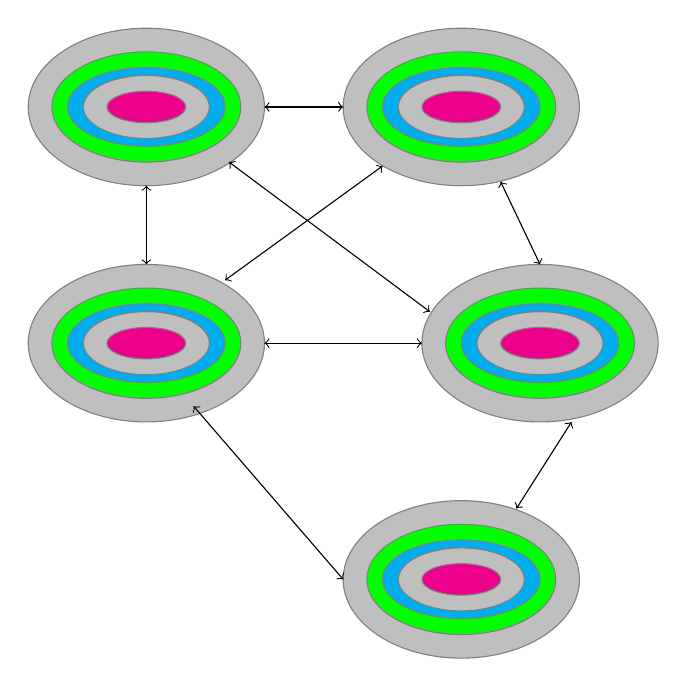
\begin{tikzpicture}

%1
\filldraw[draw=gray,fill=lightgray] (0,3) ellipse (1.5 and 1);
\filldraw[draw=gray,fill=green] (0,3) ellipse (1.2 and 0.7);
\filldraw[draw=gray,fill=cyan] (0,3) ellipse (1 and 0.5);
\filldraw[draw=gray,fill=lightgray] (0,3) ellipse (0.8 and 0.4);
\filldraw[draw=gray,fill=magenta] (0,3) ellipse (0.5 and 0.2);

%2
\filldraw[draw=gray,fill=lightgray] (0,0) ellipse (1.5 and 1);
\filldraw[draw=gray,fill=green] (0,0) ellipse (1.2 and 0.7);
\filldraw[draw=gray,fill=cyan] (0,0) ellipse (1 and 0.5);
\filldraw[draw=gray,fill=lightgray] (0,0) ellipse (0.8 and 0.4);
\filldraw[draw=gray,fill=magenta] (0,0) ellipse (0.5 and 0.2);

%3
\filldraw[draw=gray,fill=lightgray] (5,0) ellipse (1.5 and 1);
\filldraw[draw=gray,fill=green] (5,0) ellipse (1.2 and 0.7);
\filldraw[draw=gray,fill=cyan] (5,0) ellipse (1 and 0.5);
\filldraw[draw=gray,fill=lightgray] (5,0) ellipse (0.8 and 0.4);
\filldraw[draw=gray,fill=magenta] (5,0) ellipse (0.5 and 0.2);

%4
\filldraw[draw=gray,fill=lightgray] (4,3) ellipse (1.5 and 1);
\filldraw[draw=gray,fill=green] (4,3) ellipse (1.2 and 0.7);
\filldraw[draw=gray,fill=cyan] (4,3) ellipse (1 and 0.5);
\filldraw[draw=gray,fill=lightgray] (4,3) ellipse (0.8 and 0.4);
\filldraw[draw=gray,fill=magenta] (4,3) ellipse (0.5 and 0.2);

%5
\filldraw[draw=gray,fill=lightgray] (4,-3) ellipse (1.5 and 1);
\filldraw[draw=gray,fill=green] (4,-3) ellipse (1.2 and 0.7);
\filldraw[draw=gray,fill=cyan] (4,-3) ellipse (1 and 0.5);
\filldraw[draw=gray,fill=lightgray] (4,-3) ellipse (0.8 and 0.4);
\filldraw[draw=gray,fill=magenta] (4,-3) ellipse (0.5 and 0.2);

\draw[<->] (1.5,3)--(2.5,3);
\draw[<->] (0,2)--(0,1);
\draw[<->] (1.05,2.3)--(3.6,0.4);
\draw[<->] (4.5,2.05)--(5,1);
\draw[<->] (3,2.25)--(1,0.8);
\draw[<->] (1.5,0)--(3.5,0);
\draw[<->] (0.6,-0.8)--(2.5,-3);
\draw[<->] (5.4,-1)--(4.7,-2.1);
\end{tikzpicture}
\end{figure}

\chapter{服务器、工作站、终端机}

服务器(Server)是提供Internet的一种以上的网络服务的主机,例如Yahoo!提供的是WWW的服务,那么Yahoo! 就可以称之为服务器了。必须要清楚的知道,服务器是有规模大小之分的。

基本上,工作站(Workstation)可以视为仅提供特定用户,作为数值分析、科学计算的机器。而工作站与服务器的差别,大概就在于有没有提供Internet上面的服务而已,例如,如果将Sun上面的mail server开启之后,那么这部机器就可以称之为服务器了,同时也是工作站,当然,更广义的定义是,只要是没有对Internet上面提供网络服务的,那就是工作站了,这当然也就包含所谓的终端机。

简单的说,终端机(Terminal)就是end-user前面的那台电脑,例如使用一台工作机连上主机来工作,那么这一台电脑就可以称为终端机。不过,更狭义的来说,『终端机』本身应该是不具备任何可以操作的软件的,在终端机上面一定要连上服务器之后,才能进行各项操作,那才是最狭义的终端机,例如前面说过的早期的大型主机连线模式。

\chapter{嵌入式系统}

伴随传统的计算机和计算系统发展起来的,还有使用集成电路(或芯片)来运行或控制各种设备的技术,这种计算技术称为嵌入式系统(embedded system),虽然芯片不是真正意义上的计算机,但是它们确实是过去50年中技术革命的产物。

\chapter{并行计算}

在过去的40年中,计算机的变化主要是速度和基础电路的构成法,而von Neumann设计的基本体系结构却保持不变。

20世纪80年代和90年代,业界开始突破已有的von Neumann体系结构,推出了具有多处理器的商用并行计算机,它们一般可以分为两类:共享存储器系统类型和分布式存储器系统类型。

计算发展的一个明显的趋势是集中式的服务器将被计算机网络所替代,这些由网络连接的、廉价但功能强大的台式机能形成极强的运算能力。约在1990年,功能强大的个人计算机和工作站局域网(LAN)开始替代大型机和小型机,这些单独的台式机很快就用广域网(WAN)连接成更大的计算机联合体。在系统结构方面,并行处理技术、多机系统、分布式计算机系统和计算机网络以及非von Neumann系统结构开始出现。

因特网的普及又推进了网络计算和网格计算,网格是一种地域分布式计算平台,它们将能提供可信赖、一致而且廉价的对高端计算设施的访问。

在软件方面,发展为分布式操作系统、数据库和知识库系统、高效可靠的高级语言以及软件工程标准化等,并逐渐形成软件产业。

20世纪80年代末,新的体系结构已经出现,使用并行体系结构的计算机依靠的是一套互相连接的中央处理器。

一种并行机器的组织结构是所有处理器共享同一个存储部件,另一种组织结构是每个中央处理器具有自己的本地内存,与其他处理器通过高速内部网络进行通信。

并行体系结构提供了几种加快执行速度的方法,例如,把程序中的一步操作分成多个片段,在几个独立的处理器上同时执行这些程序片段,这种机器称为SIMD(单指令多数据流,single-instruction,multiple-data-stream)计算机。

第二种机器可以同时运行程序的不同部分,这种机器被称为MIMD(多指令多数据流,multiple-instruction,multiple-data-stream)计算机。

并行计算机的软件设计不同于一个计算机序列的软件设计,程序设计员必须重新考虑解决问题的方法,利用并行性进行程序设计。

\chapter{连网}

计算发展的一个明显趋势是集中式的服务器将为计算机网络所替代,这些由网络连接的、廉价但功能强大的机器能形成极强的计算能力。约在1990年,功能强大的个人计算机和工作站局域网(LAN)开始替代大型机和小型机,而这些单独的机器很快就用广域网(WAN)连接成更大的计算联合体。

20世纪80年代,多用户大型机被小型机器连接成的网络代替,这些小型机器通过连网共享打印机、软件和数据等资源。1973年由Robert Metcalfe和David Boggs发明的以太网是一种廉价的同轴电缆和一套能够让机器互相通信的协议。

工作站的设计是为了连网,1985年更高级的Intel芯片面世后,可以对个人计算机连网,1989年,Novell Netware用文件服务器把PC连接在一起,而把工作站或PC连接成网络,就形成了LAN(局域网,Local Area Network)。

Internet是从ARPANET演化而来的,ARPANET网络由11个节点构成,集中分布在Los Angeles和Boston地区。与ARPANET和LAN一样,Internet使用包交换的方法共享信息,但是,Internet由分布在世界各地的不同网络组成,这些网络之间采用通用的TCP/IP(Transmission-Control Protocol/Internet Protocol,传输控制协议/网络协议)协议通信,而协议是一套规定必须严格遵守的规则和(交互信息的)过程的代码,在计算机网络中使用协议来表示计算机交互时使用的正确规定。

\begin{verbatim}
“如果20世纪90年代的Internet是信息高速公路,那么说来,以太网就是支持它的慢车道,两者同等重要,Internet是由ARPA研究演化来的全球网络,在Xerox公司发明本地以太网前,Internet已经存在了,但是在Internet盛行之前,以太网改变了办公室计算和个人计算的本性。”
\end{verbatim}

\begin{flushright}
 ——《现代计算史》(A History of Modern Computing.Paul E.Ceruzzi)
\end{flushright}

Internet的普及使网络计算以及网格计算变得更加引人入胜。网格是一种地域分布式计算平台,它们将能提供可信赖、一致而且廉价的对高端计算设施的访问。

\chapter{计算机系统的层次结构}

用户使用高级语言编写源程序后,输入计算机中,会输出正确的结果或错误提示等,这对用户来说,计算机好像能直接执行高级语言,其实并非如此。

我们把好像能直接执行高级语言的机器称为虚拟机,实际上,用高级语言编写的源程序经过机器编译成某种中间语言程序,然后再将这个中间语言程序翻译成机器能直接用硬件实现的目标程序,机器再执行目标程序得出计算结果。

若用户用汇编语言编制程序,输入机器中也须将汇编语言源程序经过汇编程序翻译成机器能直接用硬件实现的目标程序,然后再由机器执行目标程序,这样,对用户来说,就存在一个汇编语言虚拟机。可见,不同层次的程序设计语言对应不同层次的虚拟机,于是把虚拟机和它对应的机器语言一起称为计算机系统中的一级。

计算机指令系统是能直接用硬件实现的、人与机器进行通讯的语言,因此,指令系统就是机器语言,对应机器语言的机器就是实际计算机。目前,一般计算机多采用微程序控制技术,它使每条机器指令由一串微指令(微程序)来实现,而微指令所执行的基本微操作直接由硬件来实现,因此,对于微程序计算机,用机器语言(指令系统)编写的程序是通过微程序解释来实现的,所以,微程序级是计算机系统层次结构中最基本的层次。

计算机系统按照程序设计语言的层次来划分它的层级如下图所示:

\begin{figure}[htbp]
\centering
\caption{计算机按照程序设计语言进行层级划分}
\begin{tikzpicture}

\tikzset{
box/.style={rectangle,rounded corners=5pt,minimum width=100pt,minimum height=20pt,inner sep=5pt,draw=gray,fill=lightgray}
}

\node[box] (microprogram) at (0,0) {微程序机器级};
\node[box] (machine) at (0,2) {实际机器级};
\node[box] (assembly-language) at (0,4) {汇编语言虚拟机};
\node[box] (high-language) at (0,6) {高级语言虚拟机};
\node[box] (application-language) at (0,8) {应用语言虚拟机};

\draw[->] (microprogram)--(machine);
\draw[->] (machine)--(assembly-language);
\draw[->] (assembly-language)--(high-language);
\draw[->] (high-language)--(application-language);

\node at (-3,0) {1级};
\node at (-3,2) {2级};
\node at (-3,4) {3级};
\node at (-3,6) {4级};
\node at (-3,8) {5级};

\node at (2,-0.8) {直接由硬件执行};
\node at (2,1) {解释(微程序)};
\node at (2,3) {翻译(汇编程序)};
\node at (2,5) {翻译(编译程序)};
\node at (2,7) {翻译(应用程序包)};

\end{tikzpicture}
\end{figure}

上图中1级和2级是由硬件实现的,它们是实际机器的两个层次。对于不是微程序控制的计算机,此二级合并为一级,3$\sim$5级是由软件实现的,是虚拟机器级。其中,1、2级的机器语言即微指令系统和指令系统,是面向计算机系统设计师和系统程序员的,而各虚拟机的语言是面向用户程序员的,其中,第3级汇编语言是基本符号形式语言,可以被用户直接使用,也可以作为一种中间语言存在,而4、5级高级语言更适合于用户使用。

计算机系统可以通过在若干抽象层上的接口加以定义,其中每一层将为它的上一层提供功能的支持,这些层包括应用程序、高级语言和机器指令集。根据系统不同级间的接口,就可以定义各种不同的计算机体系结构。处于应用程序和高级语言之间的接口称为语言体系结构,而指令集体系结构则定义了基本指令集与运行时间及I/O控制之间的接口。

计算机体系机构的另一个不同定义建立在四个基本概念之上,它们是结构、组成、实现和性能,其中结构定义了硬件部件之间的互连,组成定义了各个部件之间的动态相互影响和对它们的管理,实现定义了硬件部件的详细设计,而性能说明了计算机系统的行为。

\chapter{精简指令级计算机}

为了增强体系结构的性能,人们提出了关于指令集的不同的设想,其中的一个设计思想是在一条指令中做尽可能多的工作,这样就可用较少的指令数完成相同的作业,这一设计思想的直接结果是只需较少的存储器读/写操作,而获得最终的运算加速。

这一设计思想的另一个优点是,增加指令的复杂度和寻址方式具有理论上的优点,那就是可以减少高级语言指令和低级(机器)语言指令间的“语义差别”。用一条(机器)指令将十进制数(BCD)转换成二进制数是一个很好的例子,它可以说明某些指令要完成的动作有多复杂,数量众多的寻址方式又进一步增加了指令的复杂性。

追随这一设计思想的机器称为复杂指令集计算机(CISC),包括Intel Pentium、Motorola MC 68000以及IBM \& Macintosh PowerPC。

将更多的能力加到处理器,会增加支持更高时钟速率的难度,这是因为增加了在单个时钟周期内的计算复杂性,而许多研究指明,在典型的程序中,所执行的指令80 \% 以上都是那些使用赋值语句、条件转移和过程调用的指令。此外,简单赋值语句几乎占据了这些操作的50\%,这些发现便导致了另一种不同设计思想的出现。在减少指令复杂性和寻址方式的同时,该设计思想通过加速那些最常用的操作来促进体系结构的优化。
采用这一设计思想的机器称为精简指令集计算机(RISC),包括Sun SPARC、MIPS和ARM等,而研究已经证明RISC体系结构的确可以使程序更快地执行。

RISC计算机代表了计算机体系结构的重要转变。RISC强调合理分配资源来增强体系结构,从而使得执行最常用和最耗时的指令变得最为有效。基于RISC的机器可以由一些共同属性描述,比如简单而精练的指令集、固定的指令格式、一个机器周期一条指令、流水线的指令读取和执行部件、数量充足的通用寄存器(或优化的编译器代码生成),载入/存储式的存储器操作和硬连线的控制器设计。应用基本RISC原理制造的机器,包括Berkeley RISC、Stanford MIPS、Compaq Alpha和SUN UltraSparc。大多数当代的微处理器芯片均追随RISC模式。

\chapter{计算机性能衡量}

计算机的性能可以反映在不同方面。例如,用户衡量计算机的性能是基于执行一个给定作业(程序)所需的时间,而实验室工程师衡量其系统的性能则是基于在给定的时间内所完成的总工作量。用户将程序的执行时间作为性能的衡量标准,而实验室工程师则认为吞吐量是更为重要的性能衡量标准。

评估计算机性能的度量标准有助于比较不同的设计。但也明白,它们中没有一个能对一台机器的性能给以一致的定义。

性能分析应有助于回答这样的问题,即使用给定的计算机,程序能执行多快?为了回答这一问题,我们需要确定由一台计算机执行一个给定作业所需的时间。我们定义时钟周期时间为一个周期时钟信号的两个连续上升(下降)沿间的时间。时钟周期能用来为单位计算计数,因为计算结果的存储是与上升(下降)时钟沿同步的。计算机执行一个作业所需的时间通常以时钟周期数来表示。

\begin{figure}[htbp]
\centering
\begin{tikzpicture}
\draw[->](0,0)--(0,3.2);
\draw[->](0,0)--(9,0) node[below] {时间};
\draw (0.2,0.2)--(1,0.2)--(1,3)--(2,3)--(2,0.2)--(4,0.2)--(4,3)--(5,3)--(5,0.2)--(7,0.2)--(7,3)--(8,3)--(8,0.2)--(8.6,0.2);
\draw[->](2,-0.5)--(0.8,-0.5);
\draw[->](5,-0.5)--(6.2,-0.5);

\node at (3.5,-0.5) {时钟周期时间};
\end{tikzpicture}
\end{figure}

我们用CC(cycle count)表示执行一个作业所需的CPU时钟周期数,用CT(cycle time)表示周期时间,并用f = 1 / CT表示时钟频率。

由CPU执行一个作业所需的时间可表示为

\begin{center}CPU时间=CC$\times$ CT=CC/f\end{center}

\section{CPI}

计算在一个给定的程序中所执行的指令数,比计算执行该程序所需的CPU时钟周期数可能更为容易。为此,每条指令所需的平均时钟周期数(CPI,clock cycles per instruction)已作为另一种性能衡量的指标。

下面的方程说明了如何计算CPI:$$\text{CPI}=\frac{\text{程序的CPU时钟周期}}{\text{指令数}}$$
$$\text{CPU时间}=\text{指令数}\times\text{CPI}\times\text{时钟周期时间}=\frac{\text{指令数}\times\text{CPI}}{\text{时钟频率}}$$

已知一台给定机器的指令集是由ALU(简单的赋值、算术和逻辑指令)、load(装载)、store(存储)和branch(转移)等指令类型所组成,则在已知每一种指令CPI的情况下,总CPI可以用如下的公式计算。
$$\text{CPI}=\frac{\sum{}^n_{i=1}\text{CPI}_i\times \text{I}_i}{\text{指令数}}$$
其中,$\text{I}_i$是程序中执行指令类型i的次数,而$\text{CPI}_i$则表示执行这类指令所需的平均时钟周期数。

例:根据执行一组基准测试程序所记录的以下性能测量值,计算机器A的总CPI。假定CPU的时钟速率为200MHz。

\begin{table}[htbp]
\centering
\begin{tabular}{|l|l|l|}
\hline
指令类型	& 出现百分比	& 每条指令的周期数	\\
\hline
ALU		& 38		& 1			\\
\hline
load和store	& 15		& 3			\\
\hline
branch		& 42		& 4			\\
\hline
其他		& 5			& 5			\\
\hline
\end{tabular}
\end{table}

假定执行100条指令,则总CPI可计算如下:

$$\text{CPI}=\frac{\sum{}^n_{i=1}\text{CPI}_i\times \text{I}_i}{\text{指令数}}=\frac{38\times1+15\times3+42\times4+5\times5}{100}=2.76$$

注意,CPI反映的是处理器的组成和指令集的体系结构,而指令数反映的是指令集的体系结构和所使用的编译技术。这两个参数是相辅相承的,所以在评估一台给定的计算机或比较两台机器的性能时,必须同时考虑CPI和指令数两者。

\section{MIPS}

另外,受关注较多的另一个性能衡量指标是MIPS(每秒百万指令,即单位时间的指令执行速率),它定义为

$$\text{MIPS}=\frac{\text{指令数}}{\text{执行时间}\times \text{10}^6}=\frac{\text{时钟速率}}{\text{CPI}\times \text{10}^6}$$

例:假设在另一台机器B上执行前面所提及的相同基准测试程序组,所记录的测量值如下所示,现假定时钟频率为200MHz,计算机器A和机器B的MIPS。

\begin{table}[htbp]
\centering
\begin{tabular}{|l|l|l|}
\hline
指令类型	& 出现百分比	& 每条指令的周期数	\\
\hline
ALU		& 35		& 1			\\
\hline
load和store	& 30		& 2			\\
\hline
branch		& 15		& 3			\\
\hline
其他		& 20		& 5			\\
\hline
\end{tabular}
\end{table}

$$\text{CPI}_A=\frac{\sum{}^n_{i=1}\text{CPI}_i\times \text{I}_i}{\text{指令数}}=\frac{38\times1+15\times3+42\times4+5\times5}{100}=2.76$$
$$\text{MIPS}_A=\frac{\text{指令数}}{\text{执行时间}\times \text{10}^6}=\frac{\text{时钟速率}}{\text{CPI}_A\times \text{10}^6}=\frac{200\times 10^6}{2.76\times 10^6}=70.24$$
$$\text{CPI}_B=\frac{\sum{}^n_{i=1}\text{CPI}_i\times \text{I}_i}{\text{指令数}}=\frac{35\times1+30\times2+20\times5+15\times3}{100}=2.4$$
$$\text{MIPS}_B=\frac{\text{指令数}}{\text{执行时间}\times \text{10}^6}=\frac{\text{时钟速率}}{\text{CPI}_B\times \text{10}^6}=\frac{200\times 10^6}{2.4\times 10^6}=83.76$$
因此,$\text{MIPS}_B>\text{MIPS}_A$。

但是,虽然MIPS已用来衡量机器的性能,但用它比较有不同指令集的机器时必须非常小心,这是因为MIPS并不涉及执行时间。下面考虑在两台不同机器上运行一组给定的基准测试程序所得到的测量结果。

\begin{table}[htbp]
\centering
\begin{tabular}{|l|l|l|}
\hline
\multicolumn{3}{|c|}{机器A}			\\
\hline
指令类型	& 指令数(百万)	& 每条指令的周期数\\
\hline
ALU		& 8			& 1		\\
\hline
load和store	& 4			& 3		\\
\hline
branch		& 2			& 4		\\
\hline
其他		& 4			& 3		\\
\hline
\end{tabular}
\end{table}

\begin{table}[htbp]
\centering
\begin{tabular}{|l|l|l|}
\hline
\multicolumn{3}{|c|}{机器B}			\\
\hline
指令类型	& 指令数(百万)	& 每条指令的周期数\\
\hline
ALU		& 10			& 1		\\
\hline
load和store	& 8			& 2		\\
\hline
branch		& 2			& 4		\\
\hline
其他		& 4			& 3		\\
\hline
\end{tabular}
\end{table}

$$\text{CPI}_A=\frac{\sum{}^n_{i=1}\text{CPI}_i\times \text{I}_i}{\text{指令数}}=\frac{(8\times1+4\times3+2\times4+4\times3)\times 10^6}{(8+4+2+4)\times10^6}\cong 2.2$$
$$\text{MIPS}_A=\frac{\text{指令数}}{\text{执行时间}\times \text{10}^6}=\frac{\text{时钟速率}}{\text{CPI}_A\times \text{10}^6}=\frac{200\times 10^6}{2.2\times 10^6}\cong90.9$$
$$\text{CPU}_A=\frac{\text{指令数}\times \text{CPI}_A}{\text{时钟速率}}=\frac{(8+4+2+4)\times 10^6\times 2.2}{200\times10^6}=0.198s$$
$$\text{CPI}_B=\frac{\sum{}^n_{i=1}\text{CPI}_i\times \text{I}_i}{\text{指令数}}=\frac{(10\times1+8\times2+2\times4+4\times3)\times 10^6}{(10+8+2+4)\times 10^6}\cong 1.92$$
$$\text{MIPS}_B=\frac{\text{指令数}}{\text{执行时间}\times \text{10}^6}=\frac{\text{时钟速率}}{\text{CPI}_B\times \text{10}^6}=\frac{200\times 10^6}{1.92\times 10^6}\cong104.2$$
$$\text{CPU}_B=\frac{\text{指令数}\times \text{CPI}_B}{\text{时钟速率}}=\frac{(10+8+2+4)\times 10^6\times 1.92}{200\times10^6}=0.23s$$
因此$\text{MIPS}_B>\text{MIPS}_A$且$\text{CPU}_B>\text{CPU}_A$。

这个例子说明,虽然机器B比机器A有更高的MIPS,但却需要更长的CPU时间来执行相同的基准测试程序集。

\section{MFLOPS}

每秒百万次浮点运算(MFLOPS,单位时间浮点指令执行速率)也已被用来衡量机器的性能。它被定义为
$$MFLOPS=\frac{\text{程序中的浮点操作数}}{\text{执行时间}\times \text{10}^6}$$

与MIPS测量平均指令速率不同,MFLOPS只对浮点指令的子集加以定义。反对MFLOPS的一个论点基于如下事实,浮点操作集对不同机器可能是不一致的,所以确切的浮点操作将随机器的不同而不同。

另一个反对论点则基于这样的事实,即对于给定的程序,由MFLOPS衡量所得到的性能无法通用化,只能为机器提供一个单一的性能指标。而大多数用户可能对只涉及一个具体程序的机器性能不感兴趣。

综合有关更大程序集(如基准测试程序)性能的最流程方法是使用算术和几何平均,它们的定义如下:
$$\text{算术平均}=\frac{1}{\text{n}}\sum\limits^n_{i=1}\text{执行时间}$$
$$\text{几何平均}=\sqrt[n]{\prod\limits_{i=1}^n\text{执行时间}}$$
其中,执行时间i是第i个程序的执行时间,而n是基准测试程序集中的总程序数。

下面给出了计算这些指标的一个例子。

\begin{table}[htbp]
\centering
\begin{tabular}{|l|l|l|}
\hline
项		& 计算机A的CPU时间(s)	& 计算机B的CPU时间(s)	\\
\hline
程序1	& 50						& 10						\\
\hline
程序2	& 500						& 100						\\
\hline
程序3	& 5000						& 1000						\\
\hline
算术平均&1850						& 370						\\
\hline
几何平均&500						& 100						\\
\hline
\end{tabular}
\end{table}

\section{Amdahl定律}

Amdahl(阿姆达尔)定律认为是由于功率增强而导致加速($\text{SU}_0$)。在这种情况下,我们将加速作为一个指标,以衡量一台机器在实现某种功能增强后的性能相对于其原始性能的比值。下面的关系公式化了Amdahl定律。
$$\text{SU}_0=\frac{\text{增强后的性能}}{\text{增强前的性能}}$$
$$\text{加速}=\frac{\text{增强前的执行时间}}{\text{增强后的执行时间}}$$

例如,考虑对机器功能的一种可能增强,它将使某些基准测试程序的执行时间从25s减少到15s,我们就说由于执行时间的减少导致的加速为$\text{SU}_0=25/15\approx 1.67$。

在所给定的形式中,Amdahl定律所说明的情况是,功能的改进可以作用到指令执行时间。但是,有时可能获得的性能增强仅出现在部分时间$\Delta$中。在这种情况下需要推导一个新公式,以使由于部分时间$\Delta$增强而获得的加速$\text{SU}_{\Delta}$与由于整个时间的增强而获得的加速$\text{SU}_0$相关。此关系式可以表示为:
$$\text{SU}_0=\frac{1}{(1+\Delta)+(\Delta/\text{SU}_{\Delta})}$$
注意,当$\Delta$=1时,即增强在所有时间都可能时,则$\text{SU}_0=\text{SU}_{\Delta}$。

例如,考虑一台机器在实施增强措施后加速达到30,若在某些情况下,该增强仅在30\%的时间中有效的,则由于这种部分增强可三以获得的加速为:
$$\text{SU}_0=\frac{1}{(1+\Delta)+(\Delta/\text{SU}_{\Delta})}=\frac{1}{(1-0.3)+\frac{0.3}{30}}=\frac{1}{0.7+0.01}\approx1.4$$
注意,上面的公式可以通用化为如下所示的情况,即许多不同的独立增强可以分别以不同的部分时间$\Delta_1$,$\Delta_2$,···,$\Delta_n$实施,从而导致各自的加速$\text{SU}_{\Delta_1}$,$\text{SU}_{\Delta_2}$,···,$\text{SU}_{\Delta_n}$。
$$\text{SU}_0=\frac{1}{[(1-(\Delta_1+\Delta_2+\cdots+\Delta_n)]+\frac{(\Delta_1+\Delta_2+\cdots+\Delta_n)}{(\text{SU}_{\Delta_1}+\text{SU}_{\Delta_2}+\cdots+\text{SU}_{\Delta_n})}}$$





